To compare our \method to \psgd (data partition), \dsgd (sync barrier) and
\graphlab over speed of convergence and convergence quality we run
them over a collection of large real world dataset. To further demonstrate the
scalability of the approach we replicate and stack up real dataset to
artificially create datasets of terabytes scale. 

\subsection{Dataset}
We use four public datasets, two for \lda, \nytimes and
\pubmed~\footnote{\url{http://archive.ics.uci.edu/ml/datasets/Bag+of+Words}},
and one each for \dl and \mmsb,
\imagenet\footnote{\url{http://www.image-net.org/challenges/LSVRC/2010/download-public}}
and \twitter\footnote{\url{http://konect.uni-koblenz.de/networks/twitter}} respectively.
\paragraph{\nytimes} It is a collection of 300,000 Ny Times news articles that
contain 102,660 distinct words and 100,000,000 tokens (word occurrences) in the.
\paragraph{\pubmed} This set contains 8,200,000 PubMed abstracts, that have in
total 730,000,000 word occurrences and 141,043 unique words.
\paragraph{\imagenet} This dataset was originally used for large scale visual
recognition challenge in 2010~\cite{imagenet_cvpr09}. The set contains 1,261,406
images each with 1,000 features and has in total 389,080,708 non-zero pixels.
\paragraph{\twitter} This is a follower network from twitter that stores
directed edges from followers to followee~\cite{konect:twitter1}. It consists of
1,468,365,182 edges distributed among 41,652,230 vertices (users). 
\paragraph{\scaleblenytimes(\snytimes{N})} We replicate the documents in
\nytimes to create a \lda datasets that are in scales of hundreds of gigabytes. For example
\snytimes{4} is a datset that has each news article in \nytimes dataset
replicated 4 times. We create \snytimes{4}, \snytimes{16}, \snytimes{64} and
\snytimes{256} that have 1,200,000, 4,800,000, 19,200,000 and 76,800,000
documents with data sizes 6.08, 25.12, 103.4, and 421.42 gbs respectively.
Table~\ref{tab:dataset} shows the concise statistics of the dataset used in
all the experiments.

% \begin{table}
% \centering
% \begin{tabular}{c|c|c|c|} %\hline
% Dataset  & Dimensions & Non-zeros & Size \\ \hline
% \nytimes  & 300,000$\times$102,660 & 100,000,000 &  1.49 Gbs \\ \hline
% \pubmed & 8,200,000$\times$141,043 &  730,000,000 & 11.19 Gbs \\ \hline
% \imagenet & 1,261,406$\times$1,000 & 389,080,708 & 5.06 Gbs \\ \hline
% \twitter & 41,652,230$\times$41,652,230 & 1,468,365,182 & 23.99 Gbs \\ \hline
% \snytimes{4} & 1,200,000$\times$102,660 & 400,000,000 &  6.08 Gbs \\ \hline
% \snytimes{4} & 4,800,000$\times$102,660 & 1,600,000,000 &  25.12 Gbs \\ \hline
% \snytimes{4} & 19,200,000$\times$102,660 & 6,400,000,000 &  103.4 Gbs \\ \hline
% \snytimes{4} & 76.800,000$\times$102,660 & 25,600,000,000 &  421.42 Gbs \\
% \hline
% \end{tabular}
% \end{table}


\begin{table}
\centering
\scalebox{0.95}{
\begin{tabular}{c|c|c|c|} %\hline
Dataset  & Dimensions & Nonzeros & Size(GB) \\ \hline
\nytimes  & $0.3*10^6\times$102,660 & $0.1*10^9$ &  1.49  \\ \hline
\pubmed & $8.2*10^6\times$141,043 &  $0.73*10^9$ & 11.19  \\ \hline
\imagenet & $1.26*10^6\times$1,000 & $0.39*10^9$ & 5.06  \\ \hline
\twitter & $41.6*10^6\times 41.6*10^6$ & $1.5*10^9$ & 23.99 \\ \hline
\snytimes{4} & $1,2*10^6\times$102,660 & $0.4*10^9$ &  6.08  \\ \hline
\snytimes{16} & $4.8*10^6\times$102,660 & $1.6*10^9$ &  25.12  \\ \hline
\snytimes{64} & $19.2*10^6\times$102,660 & $6.4*10^9$ &  103.4  \\ \hline
\snytimes{256} & $76.8*10^6\times$102,660 & $25.6*10^9$ &  421.42  \\
\hline
\end{tabular}
}
\caption{Dimension, size and nonzero statistics for different datasets. The
exact figures are rounded off for simplicity. Size is the file size in
gigabytes. The biggest dataset (\snytimes{256}) is of size approximately 0.5
terabytes.}
\label{tab:dataset}
\end{table}


\subsection{\graphlab based solver}
We modify \graphlab's collaborative filtering toolkit to add the constraints
defined in equation~\ref{eqn:constraints} \abhi{put in the constraints
equation}, section~\ref{sec:applications}. We modify \sgd based learner of the toolkit as
it is eaisly pralleizable in the data space\abhi{Do we need to justify why we
use SGD based solver for graphlab?}.
We use its public APIs ( \textit{transform\_vertices(), periodic aggregator and map\_reduce\_vertices()}) 
to put normalization constraints. We take the simplest
and most efficient way of normalizing accross vertices. A periodic
aggregator is called after every fixed interval to compute the normalization
factor using \textit{map\_reduce\_vertices()} after which
we apply the computed factor to each vertex using \textit{transform\_vertices()}.


\begin{figure}
\centering
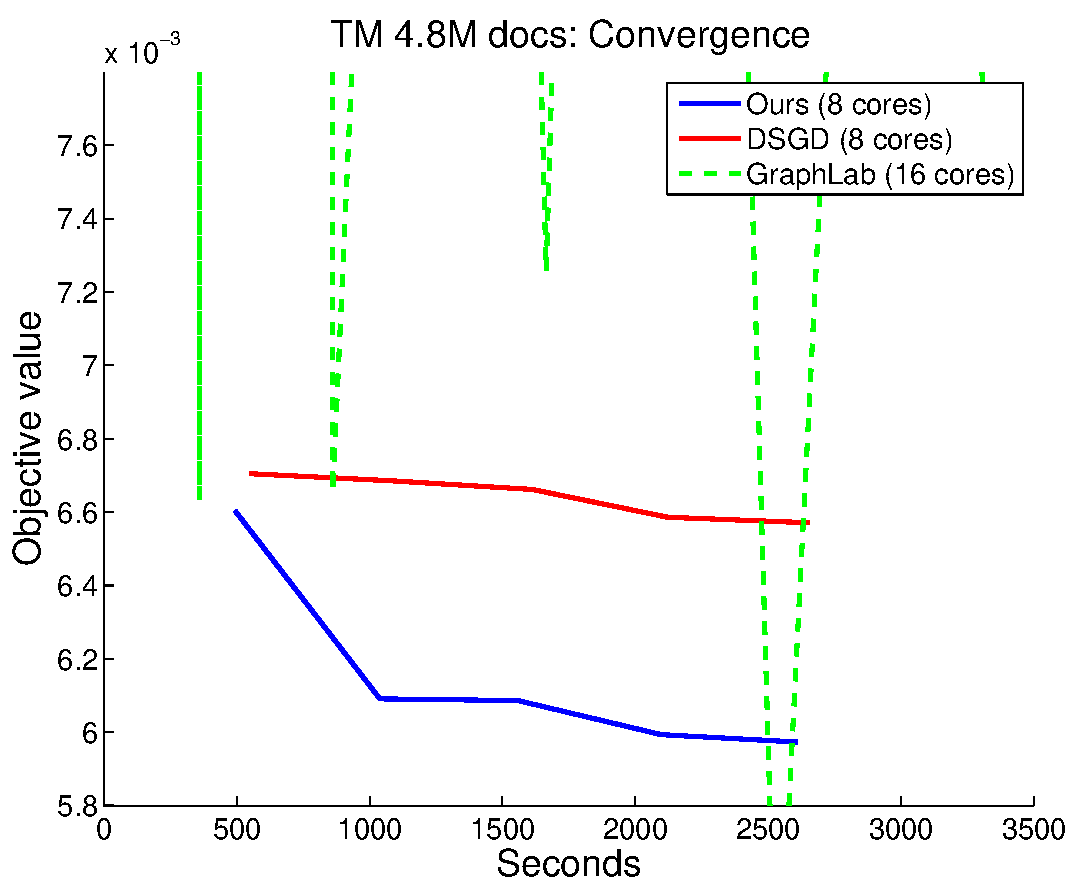
\includegraphics[width=0.46\textwidth]{results/tm_cvg.pdf} 
\label{fig:convergenceNytimes4}
\end{figure}



\begin{figure*}[t]
\centering
\begin{tabular}{|c|c|c|c|}
\hline
\multicolumn{4}{|c|}{\bf Topic Modeling} \\
\hline
Convergence Plots & \# of Topics & \# of Processors & \# of Docs \\
\hline
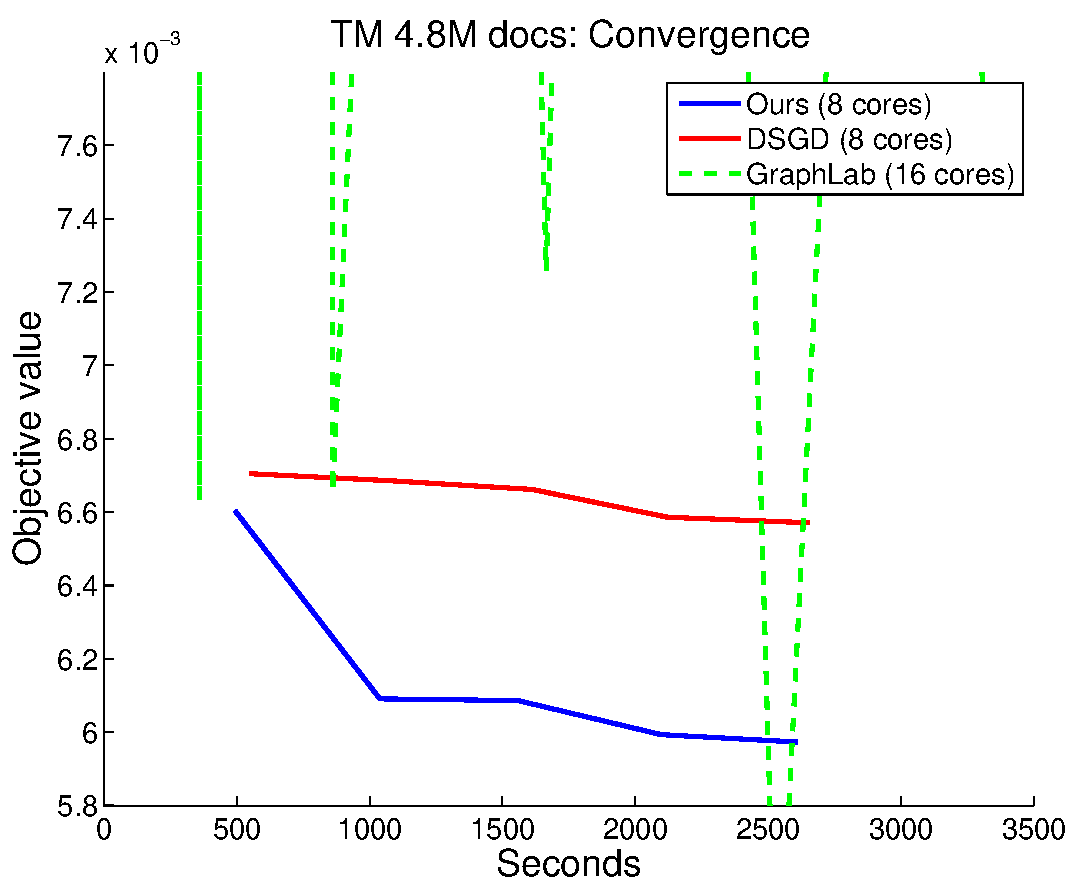
\includegraphics[width=0.23\textwidth]{results/tm_cvg.pdf} &
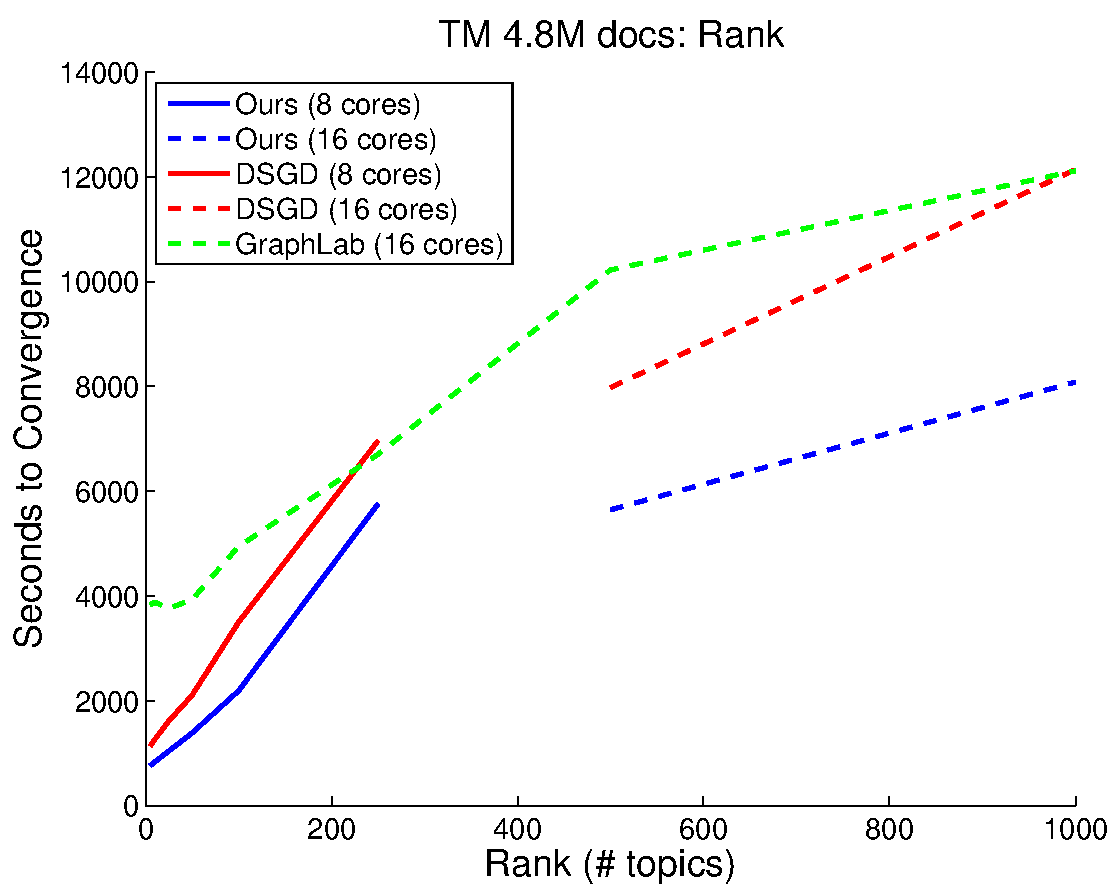
\includegraphics[width=0.23\textwidth]{results/tm_rank.pdf} &
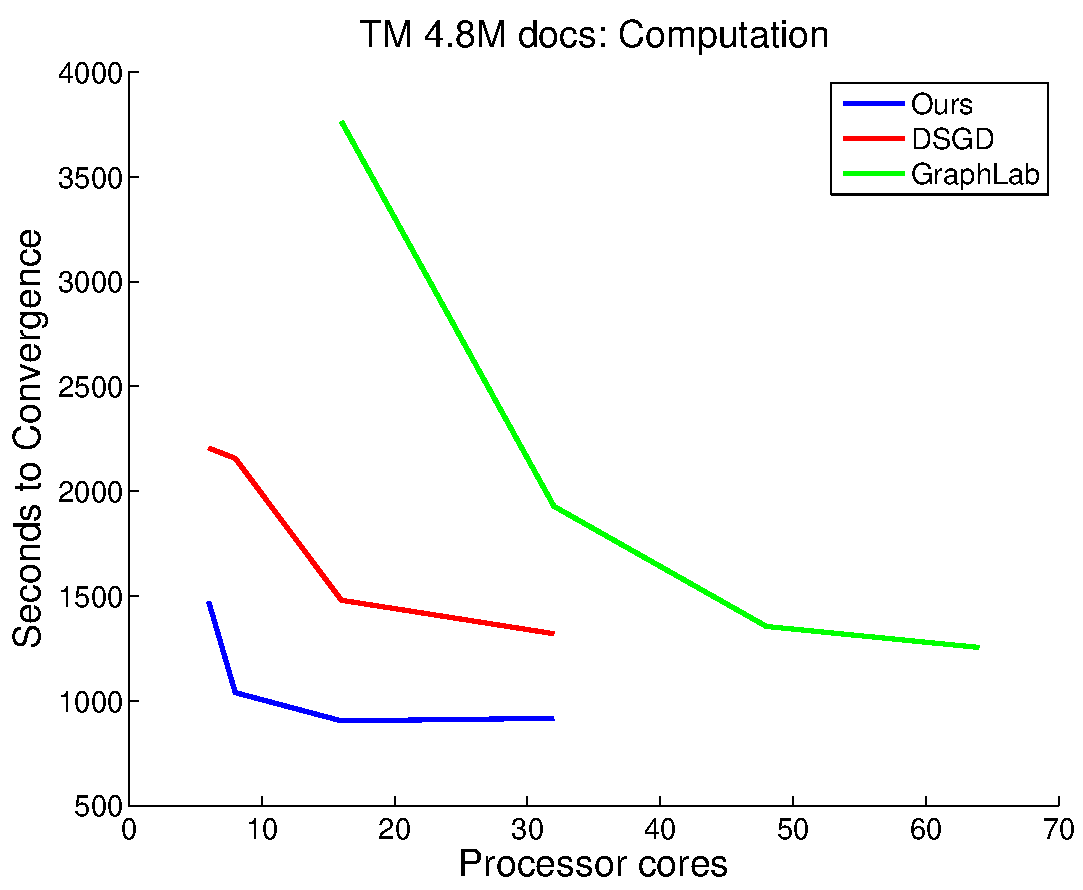
\includegraphics[width=0.23\textwidth]{results/tm_cores.pdf} &
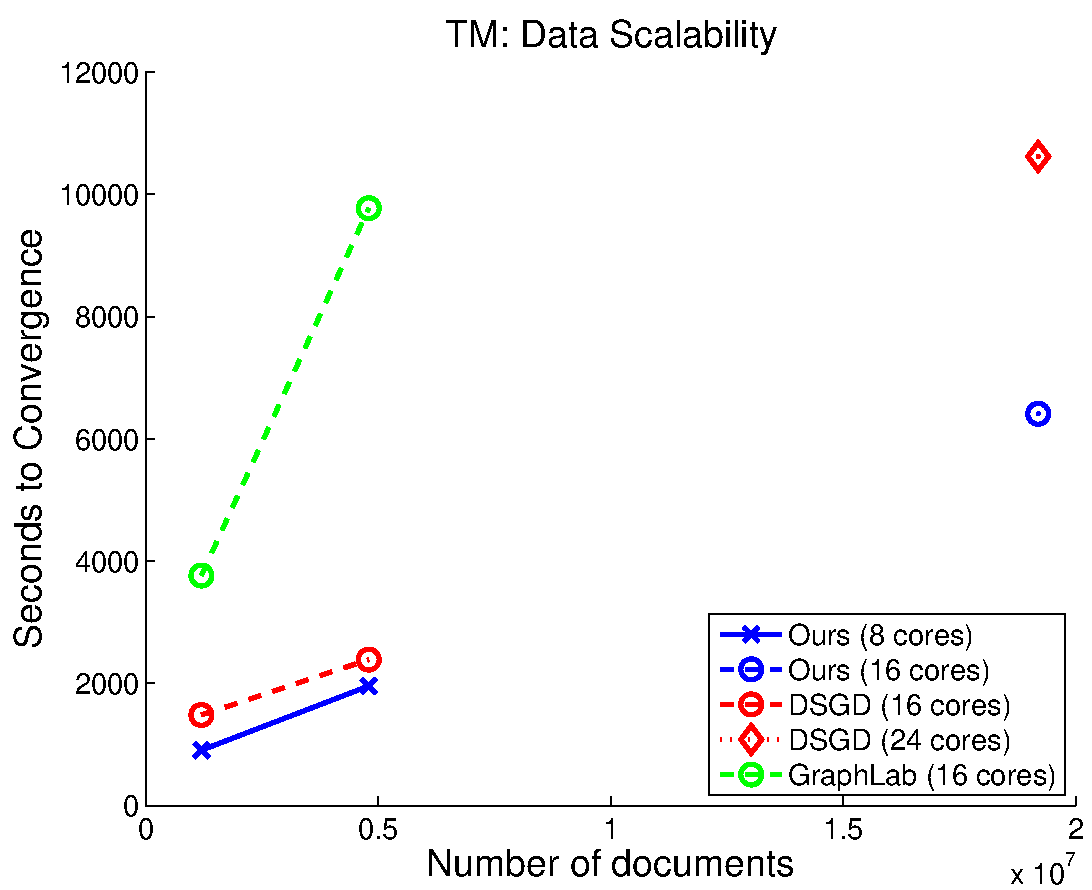
\includegraphics[width=0.23\textwidth]{results/tm_data.pdf} \\
\hline
\multicolumn{4}{|c|}{\bf Dictionary Learning} \\
\hline
Convergence Plots & \# of Dictionary Bases & \# of Processors & \# of Images \\
\hline
TODO&&&\\
\hline
\multicolumn{4}{|c|}{\bf Mixed Membership Network Decomposition} \\
\hline
Convergence Plots & \# of Network Roles & \# of Processors & \# of Network Nodes \\
\hline
TODO&&&\\
\hline
\end{tabular}
\caption{\small Convergence (Left) and scalability (in rank, processor cores and data size)
of all methods, on topic modeling, dictionary learning and mixed-membership network decomposition.
The convergence plot reveals the solution trajectory of each method, revealing pathological behavior such as oscillation.
The scalability plots show how each method fares as the problem rank, number of processor cores, and data
size is increased.}
\label{fig:results}
\end{figure*}
